\documentclass[letterpaper,11pt]{texMemo}
\usepackage[english]{babel}
\usepackage[hypcap]{caption}
\usepackage{graphicx}
\usepackage{amsmath}
\usepackage{setspace} 

\memoto{Noble Hatten}
\memofrom{Zachary Tschirhart}
\memosubject{Lab 4: Level Flight}
\memodate{March 6, 2013}

\setcounter{secnumdepth}{0}

\begin{document}
\maketitle
\doublespacing
In order to discuss the effects of altitude on an aircraft's airspeed, there is a need for a distinction between true, indicated, and equivalent airspeed to reason appropriately. In level flight, where drag is equal to the thrust and lift is equivalent to the weight of the aircraft, the velocity of an aircraft can be found by using a proportional equation,

\begin{equation}
	V_{true} = V_{equivalent} \sqrt{\frac{\rho_{Sea Level}}{\rho}}
	\label{equation:equivAirspeed}
\end{equation}

Where \(V_{equivalent}\) is the equivalent airspeed, \(V_{true}\) is the true airspeed, \(\rho\) is the density at a given altitude, and \(\rho_{Sea Level}\) is the density of air at sea level. This equation shows a proportional relationship between the two airspeeds, so as the altitude increases, the density decreases (within the experiment range), thus the equivalent airspeed decreases. Now, the relationship between the indicated airspeed and equivalent airspeed is only a difference of a constant,

\begin{equation}
    V_{indicated} = V_{equivalent} + E
	\label{equation:indiAirspeed}
\end{equation}

Where \(V_{indicated}\) is the indicated airspeed and E is the error introduced by the instrument panel. In the case of this experiment, the error will be constant throughout all of the measurements, therefore a direct conversion of indicated and equivalent can be found without the additional error factor. The recorded values in Table 1 are the indicated airspeeds at 4000 ft and 8000 ft. Using The Standard Atmosphere model, a density for sea level, 4000 ft, and 8000 ft can be found and then used to calculate the true aircraft speed relative to the atmosphere. These numbers can be seen in Tables 2 and 3. 
\\
A comparison can be made between the recorded numbers using the simulator and the numbers in Figure 1 indicating the Beechcraft performance. The difference between the indicated and true airspeed is almost identical, at full power and both altitudes. The true airspeed is actually greater than the indicated airspeed by a much larger factor at higher altitudes and the data recorded indicates that. As the manifold pressure decreased, the indicated airspeed also decreased, which again, is reflective of the data collected.
\\
As stated earlier, two of the requirements for level flight is that the thrust equals drag and lift equals the weight of the aircraft. Using this relationship, the coefficient of lift can be manipulated and substituted into the drag polar equation shown below,

\begin{equation}
   C_{L} = \frac{2W}{\rho V^2 S} 
	\label{equation:coefficentLift}
\end{equation}

Which is then substituted into the drag polar equation,

\begin{equation}
    C_D = D_{D_{O}} + K (\frac{2W}{\rho V^2 S})^2
	\label{equation:dragPolar}
\end{equation}

Where \(\rho\) is the density of the air at a given height, W is the weight of the aircraft, S is the aircraft planform area, V is the true airspeed, \(C_D\) is the coefficient of drag, and \(D_{D_{O}}\) is the coefficient of drag of zero lift. Equation 4 can be used for the parabolic drag polar and then substituted into the drag equation to get the thrust required to maintain a constant velocity,

\begin{equation}
    T_Required=D=\frac{1}{2} \rho V^2 S C_{D_{0}}+\frac{2KW^2}{\rho V^2 S}
	\label{equation:drag}
\end{equation}

This equation separates the parasitic drag and the drag of the aircraft at zero lift, which is reflected in Figure 2 by the two exponential lines on the bottom. When these two terms are summed together, a parabolic equation is created, which is also shown in Figure 2. Looking closely at this figure, the thrust will stay constant with respect to the velocity in this graph. Notice the two intersections where Drag and Thrust meet, these two intersections are known as the high and low speed solutions for the drag polar equation. The high speed solution is a stable solution, as when the plane experiences a sudden unanticipated change in velocity, the plane tends to converge back to the original velocity, because of the inverse effects of drag on the aircraft. When the perturbation tends to increase the velocity at the high speed solution, the drag is also increased while the thrust stays constant, thus decreasing the velocity until an equilibrium is met. The opposite effects are seen at the low speed solution, which is seen as an unstable solution. The recorded airspeeds during the simulation were at the high speed solution, since the low speed solution would be very difficult to stay at long enough to record anything.
\\ 
Given that the parabolic drag polar has constant coefficients and the following equation for a sample equation, 
\begin{equation}
    C_D = 0.02 + 0.07 {C_{L}}^2
	\label{equation:coeffdrag}
\end{equation}

Where \(C_{L}\) is the coefficient of lift. Using the combination of Equation 5 and 6 along with the assumption that \(\epsilon = 0\) and using the constants \(S = 181 ft^2\) and converting thrust to a horsepower, the thrust horsepower for each velocity and altitude can be shown in Table 3.


\begin{thebibliography}{0}
\bibitem{notes} Eduardo Gilden, Greg Holt, Kyle DeMars, George Jacobellis {\em ASE 167M Flight Dynamics Laboratory Flight Simulator Experiments and Computer Projects. s.l. : The University of Texas at Austin Department of Aerospace Engineering}  2012.
\end{thebibliography}
\addcontentsline{toc}{section}{Bibliography}

\section{Appendix}
\begin{table}[h]
\centering
\begin{tabular}{|l|l|l|l|l|l|l|l|l|} \hline
	{Manifold Pressure, "HG} & Max & 27 & 25 & 23 & 21 & 20 & 19 & 18\\ \hline
	{Indicated Airspeed at 4000 ft (\(ft/s\))} & 165 & 162 & 155 & 148 & 140 & 133 & 127 & 119\\ \hline
	{Indicated Airspeed at 8000 ft (\(ft/s\))} & 160 & 157 & 151 & 144 & 136 & 130 & 123 & 110\\ \hline
\end{tabular} \\
\caption{Recorded airspeeds at indicated altitudes and manifold pressures} \label{tab:Table1}
\end{table}

\begin{table}[h]
\centering
\begin{tabular}{|l|l|l|l|l|l|l|l|l|} \hline
	{Manifold Pressure, "HG} & Max & 27 & 25 & 23 & 21 & 20 & 19 & 18\\ \hline
	{True Airspeed at 4000 ft (\(ft/s\))} & 175 & 172 & 165 & 157 & 149 & 141 & 135 & 126\\ \hline
	{True Airspeed at 8000 ft (\(ft/s\))} & 181 & 177 & 170 & 162 & 153 & 147 & 139 & 124\\ \hline
\end{tabular} \\
\caption{Converted true airspeeds using the density table 3 } \label{tab:Table2}
\end{table}

\begin{table}[h]
\centering
\begin{tabular}{|l|l|} \hline
	{Density at Sea Level (\(slugs/ft^2\))} & 0.0024 \\ \hline
	{Density at 4000 ft (\(slugs/ft^2\))} & 0.0021 \\ \hline
	{Density at 8000 ft (\(slugs/ft^2\))} & 0.0019 \\ \hline
\end{tabular} \\
\caption{Density at specified altitudes using the Standard Atmosphere Model} \label{tab:Table3}
\end{table}

\begin{table}[h]
\centering
\begin{tabular}{|l|l|l|l|l|l|l|l|l|} \hline
	{Manifold Pressure, "HG} & Max & 27 & 25 & 23 & 21 & 20 & 19 & 18\\ \hline
	{Horsepower at 4000 ft (\(HP\))} & 238 & 228 & 205 & 182 & 161 & 142 & 130 & 114\\ \hline
	{Horsepower at 8000 ft (\(HP\))} & 375 & 354 & 319 & 282 & 246 & 225 & 199 & 159\\ \hline
\end{tabular} \\
\caption{True Horsepower of the engine at different altitudes} \label{tab:Table3}
\end{table}

\begin{figure}[here]
	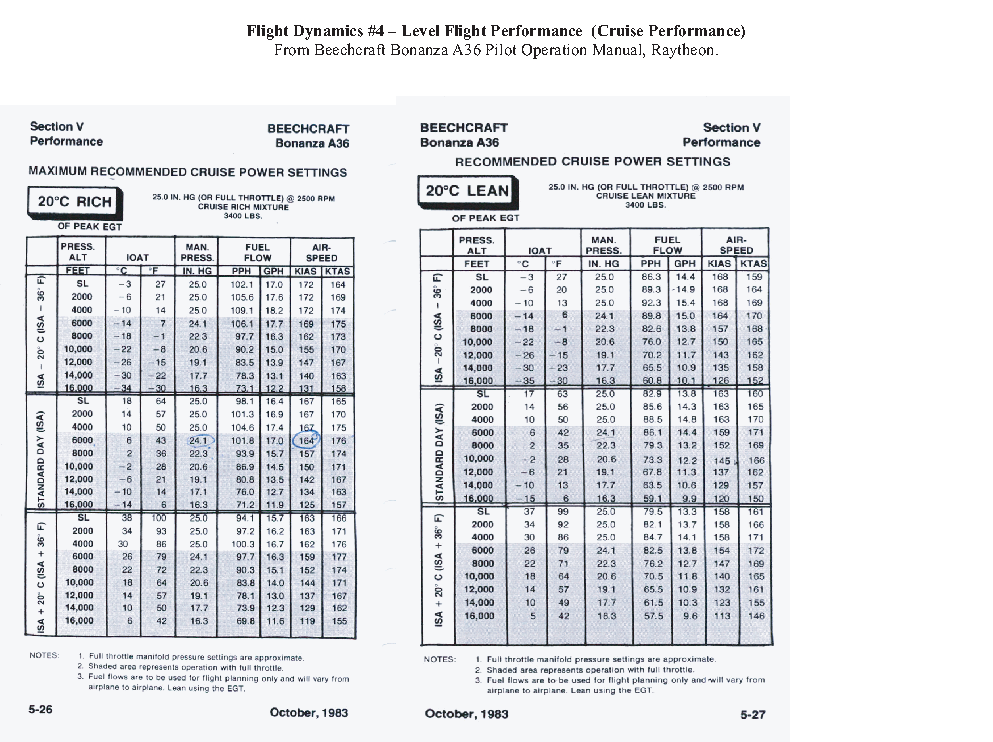
\includegraphics[width=1\textwidth]{Cruise_Performance.png}
	\caption{Beechcraft Performance measurements at various settings}
	\label{fig:Figure1}
\end{figure}

\begin{figure}[here]
	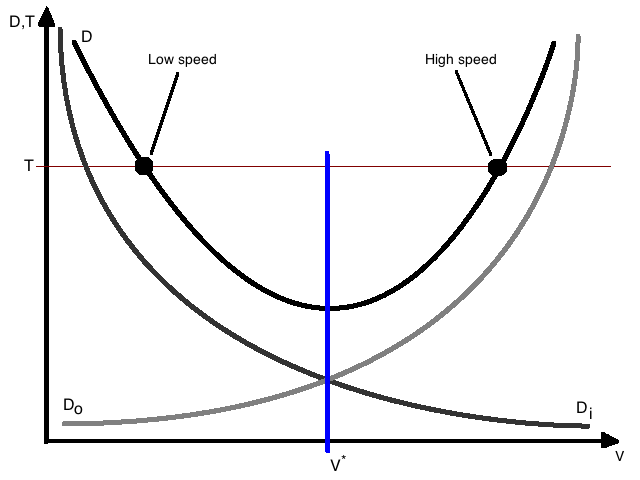
\includegraphics[width=1\textwidth]{DragPlot.png}
	\caption{Thrust and Drag versus Velocity}
	\label{fig:Figure2}
\end{figure}

\end{document}